\section{Optical flow sensor}

Optical flow sensor uses a camera to detect motion on a x and y scale. It looks for movement by finding patterns in the ground it is looking at to being able to determine in what direction and how far the rover has travelled. This is vital information for SLAM mapping. and is used for finding the next reference point. The sensor is placed high on the rover to get a bigger view of the ground and is faced downwards to the ground.

The optical flow sensor works in the same manner as your computer mouse and gives back information to the rover. What is important is the surface that the optical flow is looking at. If it is all reflecting or has differences that the camera can use for reference the reading will be wrong. It is therefore good to have a backup system like encoders on the wheels so the program knows that it is moving.


\begin{figure}[H]
	\centering
	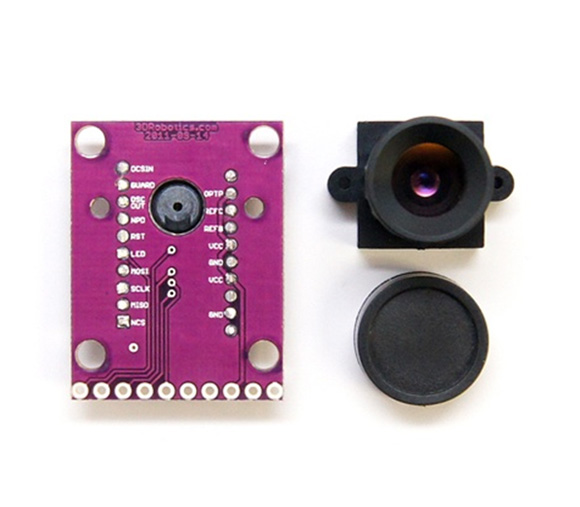
\includegraphics[width=.3\linewidth]{images/optical.jpg}
	\caption{The optical flow sensor from 3D Robotics.}
\end{figure}


%cite http://en.wikipedia.org/wiki/Optical_flow